\documentclass[border=8pt]{standalone}
\usepackage{lmodern}
\usepackage{tikz}
\usepackage{amsmath,amssymb}
\usetikzlibrary{arrows.meta,shapes.geometric,decorations.pathreplacing,calc}

\definecolor{kmblue}{HTML}{003874}
\definecolor{kmgold}{HTML}{BA9224}
\definecolor{rtgreen}{HTML}{1F9D55}
\definecolor{rtred}{HTML}{E3342F}
\definecolor{axgray}{HTML}{888888}
\definecolor{dkgray}{HTML}{333333}
\definecolor{ltbg}{HTML}{F8FAFC}
\definecolor{boxborder}{HTML}{CBD5E1}

\begin{document}
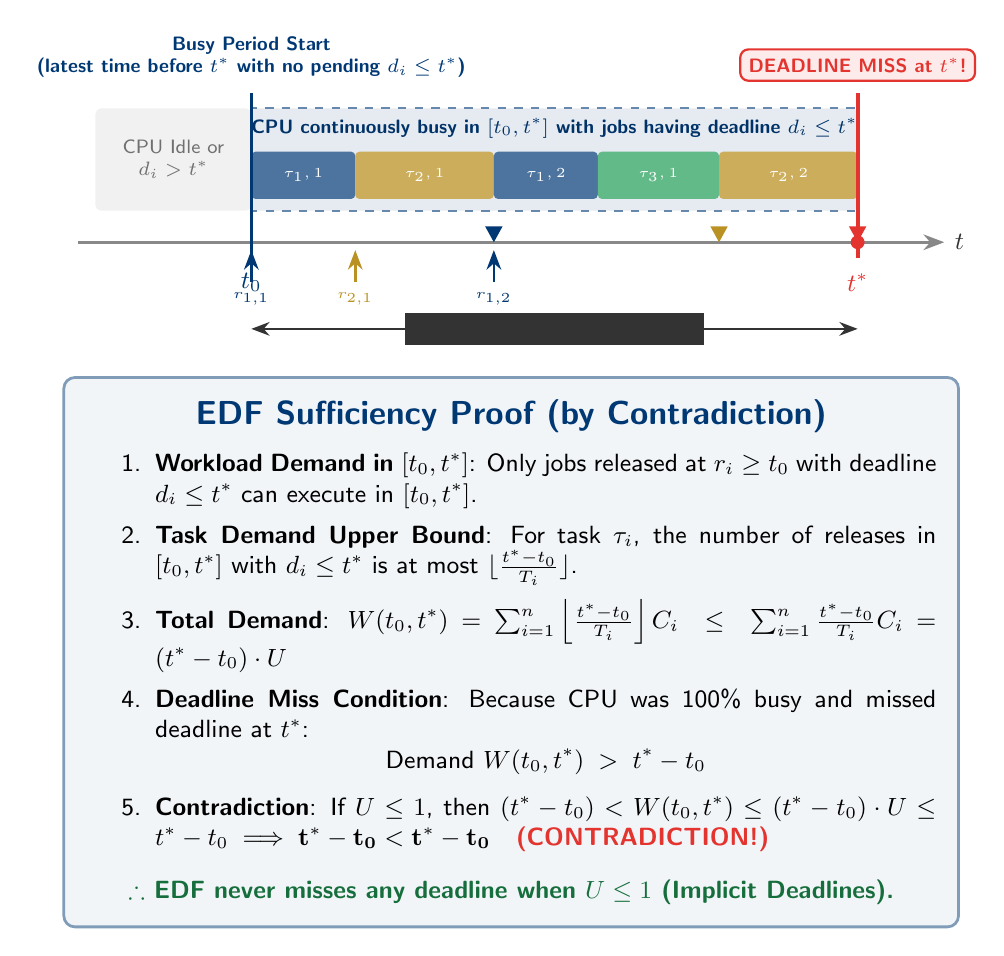
\begin{tikzpicture}[>=Stealth,font=\sffamily,x=1.1cm,y=1cm]

  % =====================================================================
  % 1. TIMELINE & BUSY PERIOD
  % =====================================================================
  
  % Idle / non-qualifying region before t0
  \fill[axgray!12,rounded corners=2pt] (-0.8, 2.5) rectangle (1.0, 3.8);
  \node[dkgray!70,font=\sffamily\scriptsize,align=center] at (0.1, 3.15)
        {CPU Idle or\\$d_i > t^*$};

  % Busy period region [t0, t*]
  \fill[kmblue!10,rounded corners=2pt] (1.0, 2.5) rectangle (8.0, 3.8);
  \draw[kmblue!60,line width=0.8pt,dashed] (1.0, 2.5) rectangle (8.0, 3.8);

  % CPU Execution blocks in [t0, t*]
  \fill[kmblue!70,rounded corners=1.5pt] (1.0, 2.65) rectangle (2.2, 3.25);
  \fill[kmgold!75,rounded corners=1.5pt] (2.2, 2.65) rectangle (3.8, 3.25);
  \fill[kmblue!70,rounded corners=1.5pt] (3.8, 2.65) rectangle (5.0, 3.25);
  \fill[rtgreen!70,rounded corners=1.5pt] (5.0, 2.65) rectangle (6.4, 3.25);
  \fill[kmgold!75,rounded corners=1.5pt] (6.4, 2.65) rectangle (8.0, 3.25);

  \node[white,font=\sffamily\tiny\bfseries] at (1.6, 2.95) {$\tau_1,1$};
  \node[white,font=\sffamily\tiny\bfseries] at (3.0, 2.95) {$\tau_2,1$};
  \node[white,font=\sffamily\tiny\bfseries] at (4.4, 2.95) {$\tau_1,2$};
  \node[white,font=\sffamily\tiny\bfseries] at (5.7, 2.95) {$\tau_3,1$};
  \node[white,font=\sffamily\tiny\bfseries] at (7.2, 2.95) {$\tau_2,2$};

  % Time axis
  \draw[axgray,line width=1.0pt,->] (-1.0, 2.1) -- (9.0, 2.1)
        node[right,font=\sffamily\small\bfseries,dkgray] {$t$};

  % t0 marker
  \draw[kmblue,line width=1.2pt] (1.0, 1.9) -- (1.0, 4.0);
  \node[below=2pt,kmblue,font=\sffamily\bfseries\small] at (1.0, 1.9) {$t_0$};
  \node[above=2pt,kmblue,font=\sffamily\scriptsize\bfseries,align=center] at (1.0, 4.0) 
        {Busy Period Start\\(latest time before $t^*$ with no pending $d_i \le t^*$)};

  % t* marker (Deadline Miss)
  \draw[rtred,line width=1.4pt] (8.0, 1.9) -- (8.0, 4.0);
  \fill[rtred] (8.0, 2.1) circle (2.5pt);
  \node[below=2pt,rtred,font=\sffamily\bfseries\small] at (8.0, 1.9) {$t^*$};
  
  % Deadline miss badge
  \node[draw=rtred,fill=rtred!10,text=rtred,rounded corners=3pt,line width=0.8pt,font=\sffamily\bfseries\scriptsize,inner sep=3pt] 
        at (8.0, 4.35) {DEADLINE MISS at $t^*$!};

  % Release arrows and deadlines within [t0, t*]
  \draw[kmblue,line width=0.9pt,->] (1.0, 1.6) -- (1.0, 2.0) node[pos=0,below,font=\sffamily\tiny] {$r_{1,1}$};
  \draw[kmgold,line width=0.9pt,->] (2.2, 1.6) -- (2.2, 2.0) node[pos=0,below,font=\sffamily\tiny] {$r_{2,1}$};
  \draw[kmblue,line width=0.9pt,->] (3.8, 1.6) -- (3.8, 2.0) node[pos=0,below,font=\sffamily\tiny] {$r_{1,2}$};

  % Deadline markers d_i <= t*
  \fill[kmblue] (3.8, 2.1) -- (3.7, 2.3) -- (3.9, 2.3) -- cycle;
  \fill[kmgold] (6.4, 2.1) -- (6.3, 2.3) -- (6.5, 2.3) -- cycle;
  \fill[rtred]  (8.0, 2.1) -- (7.9, 2.3) -- (8.1, 2.3) -- cycle;

  % Bracket for interval length (t* - t0)
  \draw[line width=0.8pt, <->, >=Stealth, dkgray] (1.0, 1.0) -- (8.0, 1.0)
        node[midway, fill=white, inner sep=2pt, font=\sffamily\small\bfseries, dkgray] 
        {Interval Duration: $t^* - t_0$};

  % CPU Busy Annotation
  \node[kmblue!90!black,font=\sffamily\scriptsize\bfseries] at (4.5, 3.55)
        {CPU continuously busy in $[t_0, t^*]$ with jobs having deadline $d_i \le t^*$};

  % =====================================================================
  % 2. CONTRADICTION PROOF SUMMARY BOX
  % =====================================================================
  
  \node[draw=kmblue!50, fill=kmblue!5, rounded corners=4pt, line width=1pt, inner sep=8pt, anchor=north] 
        at (4.0, 0.4) {
    \begin{minipage}{10.8cm}
      \centering
      \textcolor{kmblue}{\textbf{\large EDF Sufficiency Proof (by Contradiction)}} \\[4pt]
      
      \small
      \begin{enumerate}\leftmargin=1.2em \itemsep=2pt
        \item \textbf{Workload Demand in $[t_0, t^*]$}: Only jobs released at $r_i \ge t_0$ with deadline $d_i \le t^*$ can execute in $[t_0, t^*]$.
        \item \textbf{Task Demand Upper Bound}: For task $\tau_i$, the number of releases in $[t_0, t^*]$ with $d_i \le t^*$ is at most $\lfloor \frac{t^* - t_0}{T_i} \rfloor$.
        \item \textbf{Total Demand}: $W(t_0, t^*) = \sum_{i=1}^{n} \left\lfloor \frac{t^* - t_0}{T_i} \right\rfloor C_i \;\le\; \sum_{i=1}^{n} \frac{t^* - t_0}{T_i} C_i = (t^* - t_0) \cdot U$
        \item \textbf{Deadline Miss Condition}: Because CPU was 100\% busy and missed deadline at $t^*$:
              $$\text{Demand } W(t_0, t^*) \;>\; t^* - t_0$$
        \item \textbf{Contradiction}: If $U \le 1$, then $(t^* - t_0) < W(t_0, t^*) \le (t^* - t_0) \cdot U \le t^* - t_0 \implies \mathbf{t^* - t_0 < t^* - t_0} \quad \text{\textcolor{rtred}{\textbf{(CONTRADICTION!)}}}$
      \end{enumerate}
      \vspace{2pt}
      \textcolor{rtgreen!70!black}{\textbf{\small $\therefore$ EDF never misses any deadline when $U \le 1$ (Implicit Deadlines).}}
    \end{minipage}
  };

\end{tikzpicture}
\end{document}
